\cxset{
 name=CHAPTER,
 numbering=arabic,
 number font-size=\LARGE,
 number font-family=\sffamily,
 number font-weight=\bfseries,
 number before={},
 number position=rightname,
 chapter font-family=\sffamily,
 chapter font-weight=\bfseries,
 number after={},
 chapter before={\rule{\textwidth}{2pt}\par},
 chapter after={\vskip0pt\vspace*{-8pt}\rule{\textwidth}{.4pt}\vskip-7pt},
 chapter color={black!90},
 number color=black!90,
 title beforeskip={},
 title afterskip={\vspace{50pt}},
 title before=,
 title after={\par\vskip-16.5pt\rule{\textwidth}{0.4pt}\par} ,
 title font-family=\sffamily,
 title font-color=black!80,
 title font-weight=\bfseries,
 title font-size=\LARGE,
 chapter font-size=\LARGE,
 author block=false}

\chapter{STYLE 39}

This style uses rules to enclose both the chapter name and number as well as the title, which necessarily needs to be rather short.
\medskip

\begin{figure}[ht]
\centering
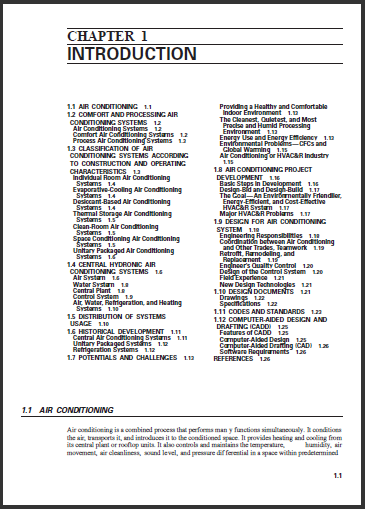
\includegraphics[width=0.6\textwidth]{./chapters/chapter39.png}
\end{figure}
In the picture it does not look very attractive, but in the actual book it does. My observation is that the rule clearances are a bit tight and if you use this type of layout it is better to experiment until you get them right.



